
% ════════════════════════════════════════════
% 模型求解（5.4.4.模型求解.tex，三级子块）
% ════════════════════════════════════════════
\subsubsection{模型求解}

基于上述模型，本节利用附件四的波动电价数据重新求解问题二与问题三（同样以 1 月为预热期、费用汇总仅统计 2 月 1 日—12 月 31 日）。该口径下波动电价问题二的购电费用为 12841054.36 元，问题三的总费用为 14956526.18 元。波动电价下问题二（对应 result4-2）四个指定日期在指定时间段的购电量及全天购电量、购电费见表\ref{tab:结果4-2a}～表\ref{tab:结果4-2d}，储能充放电量见表\ref{tab:结果4-2e}～表\ref{tab:结果4-2h}，紧急购电见表\ref{tab:结果4-2i}；波动电价下问题三（对应 result4-3）的计划购电量见表\ref{tab:结果4-3a}～表\ref{tab:结果4-3d}，储能充放电量见表\ref{tab:结果4-3e}～表\ref{tab:结果4-3h}，紧急购电见表\ref{tab:结果4-3i}。四个指定日期在波动电价下的购电费用汇总见表\ref{tab:结果4-1}。

\begin{longtable}{>{\centering\arraybackslash}p{0.15\textwidth}>{\centering\arraybackslash}p{0.13\textwidth}>{\centering\arraybackslash}p{0.15\textwidth}>{\centering\arraybackslash}p{0.13\textwidth}>{\centering\arraybackslash}p{0.15\textwidth}>{\centering\arraybackslash}p{0.13\textwidth}}
  \caption{2025.3.20 微网在指定时间段的购电量及全天的购电量和购电费}
  \label{tab:结果4-2a} \\
  \toprule
  时间段 & 购电量 & 时间段 & 购电量 & 时间段 & 购电量 \\
  \midrule
  \endfirsthead
  \caption{2025.3.20 微网在指定时间段的购电量及全天的购电量和购电费（续）} \\
  \toprule
  时间段 & 购电量 & 时间段 & 购电量 & 时间段 & 购电量 \\
  \midrule
  \endhead
  \bottomrule
  \endfoot
  10:00--10:10 & 0.00 & 12:00--12:10 & 479.31 & 14:00--14:10 & 0.00 \\
  16:00--16:10 & 562.26 & 18:00--18:10 & 0.00 & 20:00--20:10 & 0.00 \\
  全天购电量 & 66475.14 & 全天购电费 & 40946.81 &  &  \\
\end{longtable}

\begin{longtable}{>{\centering\arraybackslash}p{0.15\textwidth}>{\centering\arraybackslash}p{0.13\textwidth}>{\centering\arraybackslash}p{0.15\textwidth}>{\centering\arraybackslash}p{0.13\textwidth}>{\centering\arraybackslash}p{0.15\textwidth}>{\centering\arraybackslash}p{0.13\textwidth}}
  \caption{2025.6.21 微网在指定时间段的购电量及全天的购电量和购电费}
  \label{tab:结果4-2b} \\
  \toprule
  时间段 & 购电量 & 时间段 & 购电量 & 时间段 & 购电量 \\
  \midrule
  \endfirsthead
  \caption{2025.6.21 微网在指定时间段的购电量及全天的购电量和购电费（续）} \\
  \toprule
  时间段 & 购电量 & 时间段 & 购电量 & 时间段 & 购电量 \\
  \midrule
  \endhead
  \bottomrule
  \endfoot
  10:00--10:10 & 0.00 & 12:00--12:10 & 0.00 & 14:00--14:10 & 0.00 \\
  16:00--16:10 & 78.57 & 18:00--18:10 & 0.00 & 20:00--20:10 & 0.00 \\
  全天购电量 & 32516.29 & 全天购电费 & 15300.57 &  &  \\
\end{longtable}

\begin{longtable}{>{\centering\arraybackslash}p{0.15\textwidth}>{\centering\arraybackslash}p{0.13\textwidth}>{\centering\arraybackslash}p{0.15\textwidth}>{\centering\arraybackslash}p{0.13\textwidth}>{\centering\arraybackslash}p{0.15\textwidth}>{\centering\arraybackslash}p{0.13\textwidth}}
  \caption{2025.9.23 微网在指定时间段的购电量及全天的购电量和购电费}
  \label{tab:结果4-2c} \\
  \toprule
  时间段 & 购电量 & 时间段 & 购电量 & 时间段 & 购电量 \\
  \midrule
  \endfirsthead
  \caption{2025.9.23 微网在指定时间段的购电量及全天的购电量和购电费（续）} \\
  \toprule
  时间段 & 购电量 & 时间段 & 购电量 & 时间段 & 购电量 \\
  \midrule
  \endhead
  \bottomrule
  \endfoot
  10:00--10:10 & 0.00 & 12:00--12:10 & 354.19 & 14:00--14:10 & 0.00 \\
  16:00--16:10 & 589.43 & 18:00--18:10 & 0.00 & 20:00--20:10 & 827.18 \\
  全天购电量 & 66265.42 & 全天购电费 & 42716.48 &  &  \\
\end{longtable}

\begin{longtable}{>{\centering\arraybackslash}p{0.15\textwidth}>{\centering\arraybackslash}p{0.13\textwidth}>{\centering\arraybackslash}p{0.15\textwidth}>{\centering\arraybackslash}p{0.13\textwidth}>{\centering\arraybackslash}p{0.15\textwidth}>{\centering\arraybackslash}p{0.13\textwidth}}
  \caption{2025.12.21 微网在指定时间段的购电量及全天的购电量和购电费}
  \label{tab:结果4-2d} \\
  \toprule
  时间段 & 购电量 & 时间段 & 购电量 & 时间段 & 购电量 \\
  \midrule
  \endfirsthead
  \caption{2025.12.21 微网在指定时间段的购电量及全天的购电量和购电费（续）} \\
  \toprule
  时间段 & 购电量 & 时间段 & 购电量 & 时间段 & 购电量 \\
  \midrule
  \endhead
  \bottomrule
  \endfoot
  10:00--10:10 & 0.00 & 12:00--12:10 & 932.83 & 14:00--14:10 & 0.00 \\
  16:00--16:10 & 801.38 & 18:00--18:10 & 715.41 & 20:00--20:10 & 0.00 \\
  全天购电量 & 93611.88 & 全天购电费 & 69880.09 &  &  \\
\end{longtable}

\begin{longtable}{>{\centering\arraybackslash}p{0.15\textwidth}>{\centering\arraybackslash}p{0.13\textwidth}>{\centering\arraybackslash}p{0.13\textwidth}>{\centering\arraybackslash}p{0.15\textwidth}>{\centering\arraybackslash}p{0.13\textwidth}>{\centering\arraybackslash}p{0.13\textwidth}}
  \caption{2025.3.20 储能设备在指定时间段的充放电量及0:00和24:00的储电量}
  \label{tab:结果4-2e} \\
  \toprule
  时间段 & 充电量 & 放电量 & 时间段 & 充电量 & 放电量 \\
  \midrule
  \endfirsthead
  \caption{2025.3.20 储能设备在指定时间段的充放电量及0:00和24:00的储电量（续）} \\
  \toprule
  时间段 & 充电量 & 放电量 & 时间段 & 充电量 & 放电量 \\
  \midrule
  \endhead
  \bottomrule
  \endfoot
  00:00--04:00 & 6666.67 & 0.00 & 04:00--08:00 & 4000.00 & 5840.31 \\
  08:00--12:00 & 6291.46 & 2777.38 & 12:00--16:00 & 4662.14 & 254.72 \\
  16:00--20:00 & 0.00 & 6412.35 & 20:00--24:00 & 833.33 & 2902.65 \\
  0:00储电量 & 1200.00 &  & 24:00储电量 & 1200.00 &  \\
\end{longtable}

\begin{longtable}{>{\centering\arraybackslash}p{0.15\textwidth}>{\centering\arraybackslash}p{0.13\textwidth}>{\centering\arraybackslash}p{0.13\textwidth}>{\centering\arraybackslash}p{0.15\textwidth}>{\centering\arraybackslash}p{0.13\textwidth}>{\centering\arraybackslash}p{0.13\textwidth}}
  \caption{2025.6.21 储能设备在指定时间段的充放电量及0:00和24:00的储电量}
  \label{tab:结果4-2f} \\
  \toprule
  时间段 & 充电量 & 放电量 & 时间段 & 充电量 & 放电量 \\
  \midrule
  \endfirsthead
  \caption{2025.6.21 储能设备在指定时间段的充放电量及0:00和24:00的储电量（续）} \\
  \toprule
  时间段 & 充电量 & 放电量 & 时间段 & 充电量 & 放电量 \\
  \midrule
  \endhead
  \bottomrule
  \endfoot
  00:00--04:00 & 1666.67 & 1350.00 & 04:00--08:00 & 2123.40 & 1719.95 \\
  08:00--12:00 & 701.60 & 0.00 & 12:00--16:00 & 9965.07 & 0.00 \\
  16:00--20:00 & 0.00 & 6154.10 & 20:00--24:00 & 748.18 & 3091.92 \\
  0:00储电量 & 1200.00 &  & 24:00储电量 & 1200.00 &  \\
\end{longtable}

\begin{longtable}{>{\centering\arraybackslash}p{0.15\textwidth}>{\centering\arraybackslash}p{0.13\textwidth}>{\centering\arraybackslash}p{0.13\textwidth}>{\centering\arraybackslash}p{0.15\textwidth}>{\centering\arraybackslash}p{0.13\textwidth}>{\centering\arraybackslash}p{0.13\textwidth}}
  \caption{2025.9.23 储能设备在指定时间段的充放电量及0:00和24:00的储电量}
  \label{tab:结果4-2g} \\
  \toprule
  时间段 & 充电量 & 放电量 & 时间段 & 充电量 & 放电量 \\
  \midrule
  \endfirsthead
  \caption{2025.9.23 储能设备在指定时间段的充放电量及0:00和24:00的储电量（续）} \\
  \toprule
  时间段 & 充电量 & 放电量 & 时间段 & 充电量 & 放电量 \\
  \midrule
  \endhead
  \bottomrule
  \endfoot
  00:00--04:00 & 5833.33 & 0.00 & 04:00--08:00 & 4833.33 & 6746.77 \\
  08:00--12:00 & 5070.54 & 1896.62 & 12:00--16:00 & 6098.61 & 403.62 \\
  16:00--20:00 & 0.00 & 7021.77 & 20:00--24:00 & 0.00 & 1618.23 \\
  0:00储电量 & 1200.00 &  & 24:00储电量 & 1200.00 &  \\
\end{longtable}

\begin{longtable}{>{\centering\arraybackslash}p{0.15\textwidth}>{\centering\arraybackslash}p{0.13\textwidth}>{\centering\arraybackslash}p{0.13\textwidth}>{\centering\arraybackslash}p{0.15\textwidth}>{\centering\arraybackslash}p{0.13\textwidth}>{\centering\arraybackslash}p{0.13\textwidth}}
  \caption{2025.12.21 储能设备在指定时间段的充放电量及0:00和24:00的储电量}
  \label{tab:结果4-2h} \\
  \toprule
  时间段 & 充电量 & 放电量 & 时间段 & 充电量 & 放电量 \\
  \midrule
  \endfirsthead
  \caption{2025.12.21 储能设备在指定时间段的充放电量及0:00和24:00的储电量（续）} \\
  \toprule
  时间段 & 充电量 & 放电量 & 时间段 & 充电量 & 放电量 \\
  \midrule
  \endhead
  \bottomrule
  \endfoot
  00:00--04:00 & 9000.00 & 0.00 & 04:00--08:00 & 1666.67 & 833.33 \\
  08:00--12:00 & 5833.33 & 7806.67 & 12:00--16:00 & 7500.00 & 2220.11 \\
  16:00--20:00 & 74.21 & 5171.86 & 20:00--24:00 & 0.00 & 3468.14 \\
  0:00储电量 & 1200.00 &  & 24:00储电量 & 1200.00 &  \\
\end{longtable}

\begin{longtable}{>{\centering\arraybackslash}p{0.11\textwidth}>{\centering\arraybackslash}p{0.08\textwidth}>{\centering\arraybackslash}p{0.11\textwidth}>{\centering\arraybackslash}p{0.08\textwidth}>{\centering\arraybackslash}p{0.11\textwidth}>{\centering\arraybackslash}p{0.08\textwidth}>{\centering\arraybackslash}p{0.11\textwidth}>{\centering\arraybackslash}p{0.08\textwidth}}
  \caption{微网在指定日期的紧急购电量} \\
  \label{tab:结果4-2i} \\
  \toprule
  \multicolumn{2}{c}{2025.3.20} & \multicolumn{2}{c}{2025.6.21} & \multicolumn{2}{c}{2025.9.23} & \multicolumn{2}{c}{2025.12.21} \\
  \cmidrule(lr){1-2} \cmidrule(lr){3-4} \cmidrule(lr){5-6} \cmidrule(lr){7-8}
  时间段 & 购电量 & 时间段 & 购电量 & 时间段 & 购电量 & 时间段 & 购电量 \\
  \midrule
  \endfirsthead
  \caption{微网在指定日期的紧急购电量（续）} \\
  \toprule
  \multicolumn{2}{c}{2025.3.20} & \multicolumn{2}{c}{2025.6.21} & \multicolumn{2}{c}{2025.9.23} & \multicolumn{2}{c}{2025.12.21} \\
  \cmidrule(lr){1-2} \cmidrule(lr){3-4} \cmidrule(lr){5-6} \cmidrule(lr){7-8}
  时间段 & 购电量 & 时间段 & 购电量 & 时间段 & 购电量 & 时间段 & 购电量 \\
  \midrule
  \endhead
  \bottomrule
  \endfoot
  --- & 0.00 & --- & 0.00 & --- & 0.00 & --- & 0.00 \\
\end{longtable}

\begin{longtable}{>{\centering\arraybackslash}p{0.15\textwidth}>{\centering\arraybackslash}p{0.13\textwidth}>{\centering\arraybackslash}p{0.15\textwidth}>{\centering\arraybackslash}p{0.13\textwidth}>{\centering\arraybackslash}p{0.15\textwidth}>{\centering\arraybackslash}p{0.13\textwidth}}
  \caption{2025.3.20 微网在指定时间段的计划购电量及全天的购电量和购电费}
  \label{tab:结果4-3a} \\
  \toprule
  时间段 & 购电量 & 时间段 & 购电量 & 时间段 & 购电量 \\
  \midrule
  \endfirsthead
  \caption{2025.3.20 微网在指定时间段的计划购电量及全天的购电量和购电费（续）} \\
  \toprule
  时间段 & 购电量 & 时间段 & 购电量 & 时间段 & 购电量 \\
  \midrule
  \endhead
  \bottomrule
  \endfoot
  10:00--10:10 & 0.00 & 12:00--12:10 & 560.43 & 14:00--14:10 & 0.00 \\
  16:00--16:10 & 663.99 & 18:00--18:10 & 0.00 & 20:00--20:10 & 0.00 \\
  全天购电量 & 67887.93 & 全天购电费 & 41997.87 &  &  \\
\end{longtable}

\begin{longtable}{>{\centering\arraybackslash}p{0.15\textwidth}>{\centering\arraybackslash}p{0.13\textwidth}>{\centering\arraybackslash}p{0.15\textwidth}>{\centering\arraybackslash}p{0.13\textwidth}>{\centering\arraybackslash}p{0.15\textwidth}>{\centering\arraybackslash}p{0.13\textwidth}}
  \caption{2025.6.21 微网在指定时间段的计划购电量及全天的购电量和购电费}
  \label{tab:结果4-3b} \\
  \toprule
  时间段 & 购电量 & 时间段 & 购电量 & 时间段 & 购电量 \\
  \midrule
  \endfirsthead
  \caption{2025.6.21 微网在指定时间段的计划购电量及全天的购电量和购电费（续）} \\
  \toprule
  时间段 & 购电量 & 时间段 & 购电量 & 时间段 & 购电量 \\
  \midrule
  \endhead
  \bottomrule
  \endfoot
  10:00--10:10 & 0.00 & 12:00--12:10 & 0.00 & 14:00--14:10 & 0.00 \\
  16:00--16:10 & 111.20 & 18:00--18:10 & 0.00 & 20:00--20:10 & 0.00 \\
  全天购电量 & 33099.44 & 全天购电费 & 15620.14 &  &  \\
\end{longtable}

\begin{longtable}{>{\centering\arraybackslash}p{0.15\textwidth}>{\centering\arraybackslash}p{0.13\textwidth}>{\centering\arraybackslash}p{0.15\textwidth}>{\centering\arraybackslash}p{0.13\textwidth}>{\centering\arraybackslash}p{0.15\textwidth}>{\centering\arraybackslash}p{0.13\textwidth}}
  \caption{2025.9.23 微网在指定时间段的计划购电量及全天的购电量和购电费}
  \label{tab:结果4-3c} \\
  \toprule
  时间段 & 购电量 & 时间段 & 购电量 & 时间段 & 购电量 \\
  \midrule
  \endfirsthead
  \caption{2025.9.23 微网在指定时间段的计划购电量及全天的购电量和购电费（续）} \\
  \toprule
  时间段 & 购电量 & 时间段 & 购电量 & 时间段 & 购电量 \\
  \midrule
  \endhead
  \bottomrule
  \endfoot
  10:00--10:10 & 0.00 & 12:00--12:10 & 371.59 & 14:00--14:10 & 0.00 \\
  16:00--16:10 & 636.70 & 18:00--18:10 & 0.00 & 20:00--20:10 & 827.18 \\
  全天购电量 & 68433.17 & 全天购电费 & 44112.85 &  &  \\
\end{longtable}

\begin{longtable}{>{\centering\arraybackslash}p{0.15\textwidth}>{\centering\arraybackslash}p{0.13\textwidth}>{\centering\arraybackslash}p{0.15\textwidth}>{\centering\arraybackslash}p{0.13\textwidth}>{\centering\arraybackslash}p{0.15\textwidth}>{\centering\arraybackslash}p{0.13\textwidth}}
  \caption{2025.12.21 微网在指定时间段的计划购电量及全天的购电量和购电费}
  \label{tab:结果4-3d} \\
  \toprule
  时间段 & 购电量 & 时间段 & 购电量 & 时间段 & 购电量 \\
  \midrule
  \endfirsthead
  \caption{2025.12.21 微网在指定时间段的计划购电量及全天的购电量和购电费（续）} \\
  \toprule
  时间段 & 购电量 & 时间段 & 购电量 & 时间段 & 购电量 \\
  \midrule
  \endhead
  \bottomrule
  \endfoot
  10:00--10:10 & 0.00 & 12:00--12:10 & 979.54 & 14:00--14:10 & 0.00 \\
  16:00--16:10 & 799.69 & 18:00--18:10 & 715.41 & 20:00--20:10 & 0.00 \\
  全天购电量 & 93474.87 & 全天购电费 & 69824.09 &  &  \\
\end{longtable}

\begin{longtable}{>{\centering\arraybackslash}p{0.15\textwidth}>{\centering\arraybackslash}p{0.13\textwidth}>{\centering\arraybackslash}p{0.13\textwidth}>{\centering\arraybackslash}p{0.15\textwidth}>{\centering\arraybackslash}p{0.13\textwidth}>{\centering\arraybackslash}p{0.13\textwidth}}
  \caption{2025.3.20 储能设备在指定时间段的充放电量及0:00和24:00的储电量}
  \label{tab:结果4-3e} \\
  \toprule
  时间段 & 充电量 & 放电量 & 时间段 & 充电量 & 放电量 \\
  \midrule
  \endfirsthead
  \caption{2025.3.20 储能设备在指定时间段的充放电量及0:00和24:00的储电量（续）} \\
  \toprule
  时间段 & 充电量 & 放电量 & 时间段 & 充电量 & 放电量 \\
  \midrule
  \endhead
  \bottomrule
  \endfoot
  00:00--04:00 & 6666.67 & 0.00 & 04:00--08:00 & 4000.00 & 6149.96 \\
  08:00--12:00 & 4106.95 & 2313.92 & 12:00--16:00 & 6651.73 & 250.65 \\
  16:00--20:00 & 0.00 & 6412.35 & 20:00--24:00 & 833.33 & 2902.65 \\
  0:00储电量 & 1200.00 &  & 24:00储电量 & 1200.00 &  \\
\end{longtable}

\begin{longtable}{>{\centering\arraybackslash}p{0.15\textwidth}>{\centering\arraybackslash}p{0.13\textwidth}>{\centering\arraybackslash}p{0.13\textwidth}>{\centering\arraybackslash}p{0.15\textwidth}>{\centering\arraybackslash}p{0.13\textwidth}>{\centering\arraybackslash}p{0.13\textwidth}}
  \caption{2025.6.21 储能设备在指定时间段的充放电量及0:00和24:00的储电量}
  \label{tab:结果4-3f} \\
  \toprule
  时间段 & 充电量 & 放电量 & 时间段 & 充电量 & 放电量 \\
  \midrule
  \endfirsthead
  \caption{2025.6.21 储能设备在指定时间段的充放电量及0:00和24:00的储电量（续）} \\
  \toprule
  时间段 & 充电量 & 放电量 & 时间段 & 充电量 & 放电量 \\
  \midrule
  \endhead
  \bottomrule
  \endfoot
  00:00--04:00 & 1666.67 & 1350.00 & 04:00--08:00 & 2242.74 & 1816.62 \\
  08:00--12:00 & 1812.59 & 0.00 & 12:00--16:00 & 8839.57 & 0.00 \\
  16:00--20:00 & 14.50 & 6154.10 & 20:00--24:00 & 748.18 & 3091.92 \\
  0:00储电量 & 1200.00 &  & 24:00储电量 & 1200.00 &  \\
\end{longtable}

\begin{longtable}{>{\centering\arraybackslash}p{0.15\textwidth}>{\centering\arraybackslash}p{0.13\textwidth}>{\centering\arraybackslash}p{0.13\textwidth}>{\centering\arraybackslash}p{0.15\textwidth}>{\centering\arraybackslash}p{0.13\textwidth}>{\centering\arraybackslash}p{0.13\textwidth}}
  \caption{2025.9.23 储能设备在指定时间段的充放电量及0:00和24:00的储电量}
  \label{tab:结果4-3g} \\
  \toprule
  时间段 & 充电量 & 放电量 & 时间段 & 充电量 & 放电量 \\
  \midrule
  \endfirsthead
  \caption{2025.9.23 储能设备在指定时间段的充放电量及0:00和24:00的储电量（续）} \\
  \toprule
  时间段 & 充电量 & 放电量 & 时间段 & 充电量 & 放电量 \\
  \midrule
  \endhead
  \bottomrule
  \endfoot
  00:00--04:00 & 5833.33 & 0.00 & 04:00--08:00 & 4833.33 & 6435.18 \\
  08:00--12:00 & 5130.10 & 1920.52 & 12:00--16:00 & 5575.59 & 315.91 \\
  16:00--20:00 & 0.00 & 7021.77 & 20:00--24:00 & 0.00 & 1618.23 \\
  0:00储电量 & 1200.00 &  & 24:00储电量 & 1200.00 &  \\
\end{longtable}

\begin{longtable}{>{\centering\arraybackslash}p{0.15\textwidth}>{\centering\arraybackslash}p{0.13\textwidth}>{\centering\arraybackslash}p{0.13\textwidth}>{\centering\arraybackslash}p{0.15\textwidth}>{\centering\arraybackslash}p{0.13\textwidth}>{\centering\arraybackslash}p{0.13\textwidth}}
  \caption{2025.12.21 储能设备在指定时间段的充放电量及0:00和24:00的储电量}
  \label{tab:结果4-3h} \\
  \toprule
  时间段 & 充电量 & 放电量 & 时间段 & 充电量 & 放电量 \\
  \midrule
  \endfirsthead
  \caption{2025.12.21 储能设备在指定时间段的充放电量及0:00和24:00的储电量（续）} \\
  \toprule
  时间段 & 充电量 & 放电量 & 时间段 & 充电量 & 放电量 \\
  \midrule
  \endhead
  \bottomrule
  \endfoot
  00:00--04:00 & 9000.00 & 0.00 & 04:00--08:00 & 1666.67 & 835.79 \\
  08:00--12:00 & 5833.33 & 7547.60 & 12:00--16:00 & 7500.00 & 2432.26 \\
  16:00--20:00 & 19.32 & 5171.86 & 20:00--24:00 & 0.00 & 3468.14 \\
  0:00储电量 & 1200.00 &  & 24:00储电量 & 1200.00 &  \\
\end{longtable}

\begin{longtable}{>{\centering\arraybackslash}p{0.11\textwidth}>{\centering\arraybackslash}p{0.08\textwidth}>{\centering\arraybackslash}p{0.11\textwidth}>{\centering\arraybackslash}p{0.08\textwidth}>{\centering\arraybackslash}p{0.11\textwidth}>{\centering\arraybackslash}p{0.08\textwidth}>{\centering\arraybackslash}p{0.11\textwidth}>{\centering\arraybackslash}p{0.08\textwidth}}
  \caption{微网在指定日期的紧急购电量} \\
  \label{tab:结果4-3i} \\
  \toprule
  \multicolumn{2}{c}{2025.3.20} & \multicolumn{2}{c}{2025.6.21} & \multicolumn{2}{c}{2025.9.23} & \multicolumn{2}{c}{2025.12.21} \\
  \cmidrule(lr){1-2} \cmidrule(lr){3-4} \cmidrule(lr){5-6} \cmidrule(lr){7-8}
  时间段 & 购电量 & 时间段 & 购电量 & 时间段 & 购电量 & 时间段 & 购电量 \\
  \midrule
  \endfirsthead
  \caption{微网在指定日期的紧急购电量（续）} \\
  \toprule
  \multicolumn{2}{c}{2025.3.20} & \multicolumn{2}{c}{2025.6.21} & \multicolumn{2}{c}{2025.9.23} & \multicolumn{2}{c}{2025.12.21} \\
  \cmidrule(lr){1-2} \cmidrule(lr){3-4} \cmidrule(lr){5-6} \cmidrule(lr){7-8}
  时间段 & 购电量 & 时间段 & 购电量 & 时间段 & 购电量 & 时间段 & 购电量 \\
  \midrule
  \endhead
  \bottomrule
  \endfoot
  06:00--12:00 & 2497.25 & 04:00--04:50 & 2.34 & 06:00--06:50 & 692.04 & 07:00--08:10 & 67.18 \\
  12:30--14:20 & 545.00 & 05:00--05:30 & 12.59 & 07:10--08:00 & 61.88 & 08:50--12:00 & 829.59 \\
  14:40--15:10 & 35.16 & 06:00--06:10 & 154.67 & 08:10--09:00 & 64.49 & 13:00--13:10 & 2.28 \\
  15:20--16:20 & 119.81 & 06:20--07:20 & 343.81 & 09:50--10:20 & 46.53 & 16:30--16:50 & 13.69 \\
  16:50--17:50 & 77.14 & 13:00--13:10 & 1.48 & 10:40--11:00 & 48.04 &  &  \\
   &  & 16:00--16:20 & 5.78 & 11:40--12:00 & 57.68 &  &  \\
   &  & 17:20--17:30 & 0.50 & 12:50--14:00 & 121.33 &  &  \\
   &  & 19:00--19:50 & 2.58 & 14:20--15:00 & 92.64 &  &  \\
   &  &  &  & 15:50--16:30 & 24.37 &  &  \\
   &  &  &  & 17:00--17:50 & 64.93 &  &  \\
\end{longtable}

\begin{longtable}{>{\centering\arraybackslash}p{0.21\textwidth}>{\centering\arraybackslash}p{0.23\textwidth}>{\centering\arraybackslash}p{0.23\textwidth}>{\centering\arraybackslash}p{0.21\textwidth}}
  \caption{波动电价下指定日期的购电费用}
  \label{tab:结果4-1} \\
  \toprule
  日期 & 问题二购电费 & 问题三总费用 & 紧急购电费 \\
  \midrule
  \endfirsthead
  \caption{波动电价下指定日期的购电费用（续）} \\
  \toprule
  日期 & 问题二购电费 & 问题三总费用 & 紧急购电费 \\
  \midrule
  \endhead
  \bottomrule
  \endfoot
  2025.3.20 & 40946.81 & 54192.97 & 13666.00 \\
  2025.6.21 & 15300.57 & 17963.88 & 1618.00 \\
  2025.9.23 & 42716.48 & 49152.77 & 5928.00 \\
  2025.12.21 & 69880.09 & 75009.33 & 4147.00 \\
\end{longtable}

波动电价下四季典型日的购电功率策略如图\ref{fig:结果4-2}所示。与固定电价情形相比，购电功率对电价波动的响应更加灵敏，夜间低电价时段的购电与充电功率明显增大，白天高电价时段的购电被进一步压缩，体现了波动电价下更为积极的低充高放套利行为。

\begin{figure}[H]
    \centering
    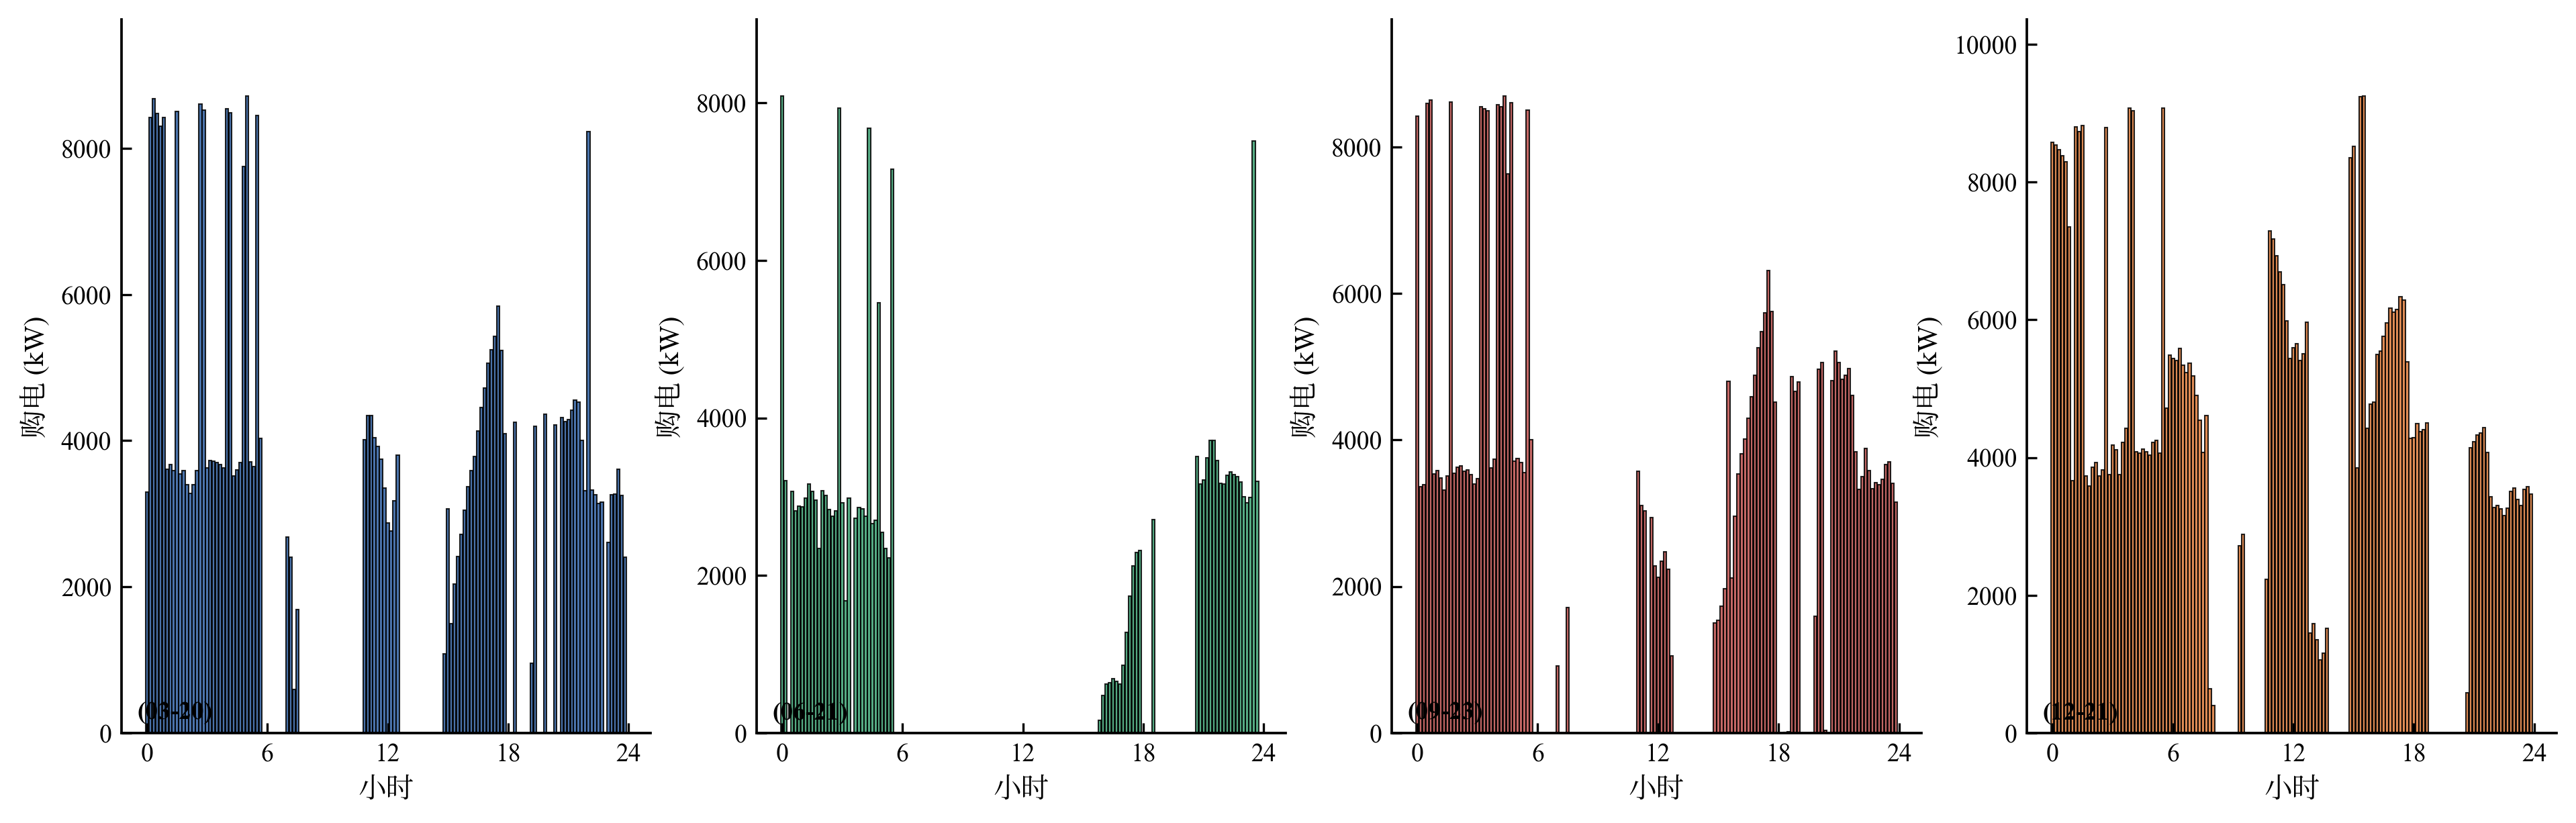
\includegraphics[width=0.75\textwidth]{../求解/问题四/图片/图4-2_波动电价四季典型日购电.png}
    \caption{波动电价下四季典型日购电策略}
    \label{fig:结果4-2}
\end{figure}

波动电价下典型日的计划购电与滚动调整购电对比如图\ref{fig:结果4-3}所示。调整策略依然能够在光伏预报更新的时点及时修正购电功率，但由于电价本身波动，调整幅度与固定电价情形存在差异，总体上仍以减小供电缺口、降低高价时段购电为目标。

\begin{figure}[H]
    \centering
    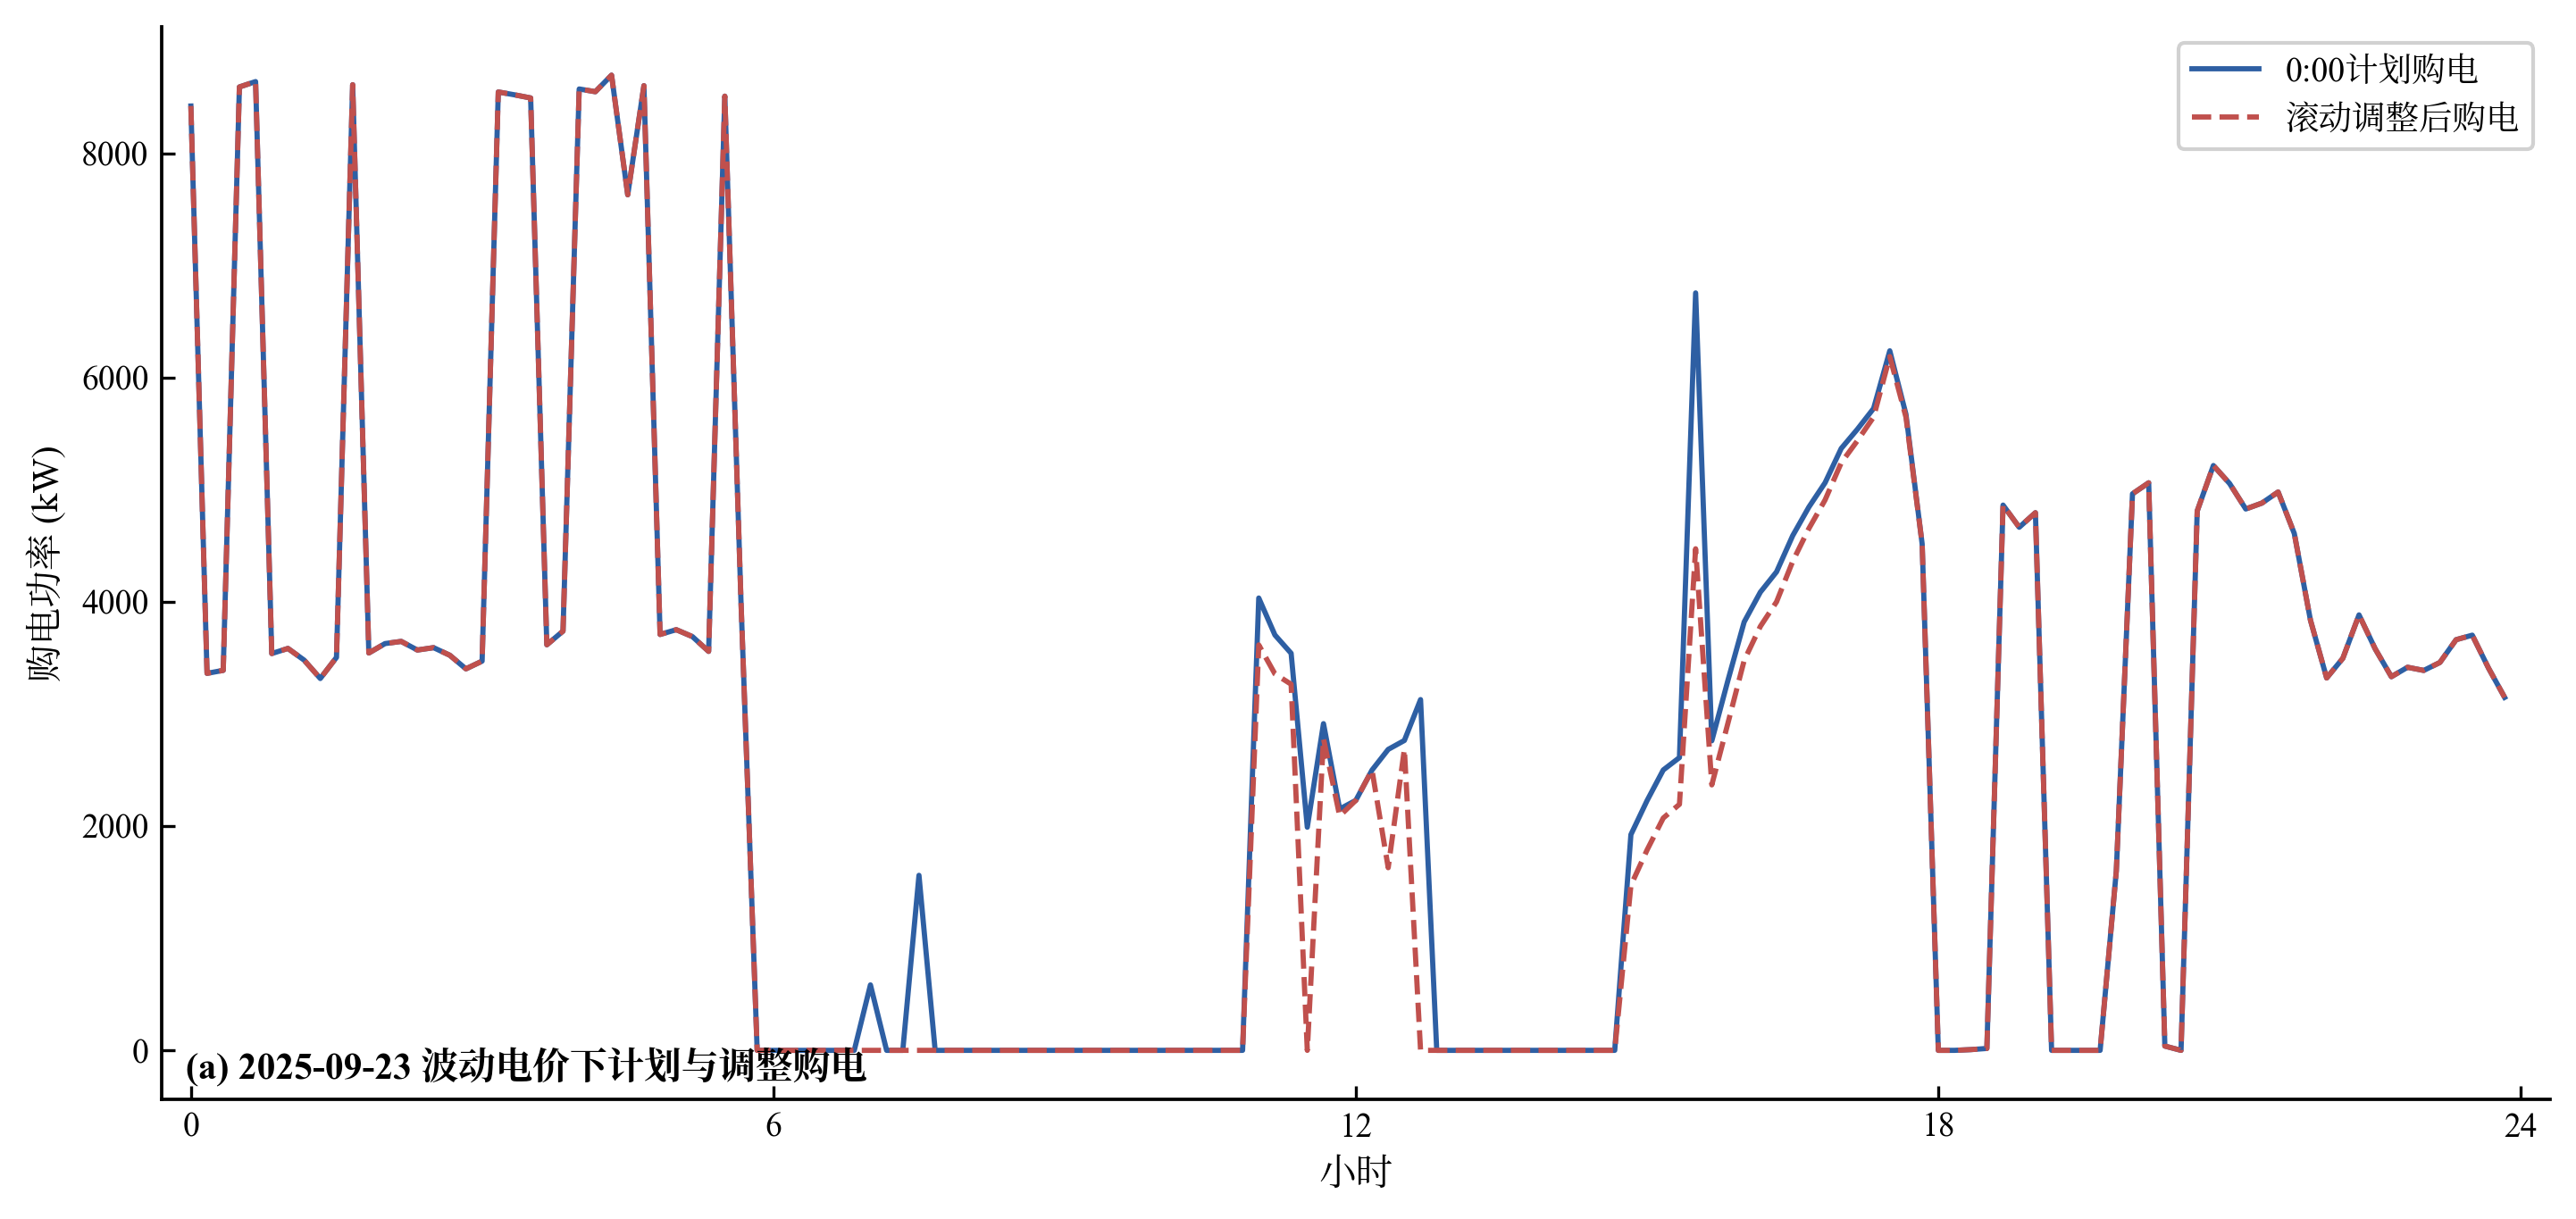
\includegraphics[width=0.70\textwidth]{../求解/问题四/图片/图4-3_波动电价滚动调整购电.png}
    \caption{波动电价下典型日计划与调整购电对比}
    \label{fig:结果4-3}
\end{figure}

波动电价下典型日的储能荷电状态轨迹如图\ref{fig:结果4-4}所示。储能荷电状态在一天内完成多次充放切换，以适应波动电价的峰谷变化，且全程满足容量约束，说明储能能够有效利用波动电价的峰谷价差获取套利收益。

\begin{figure}[H]
    \centering
    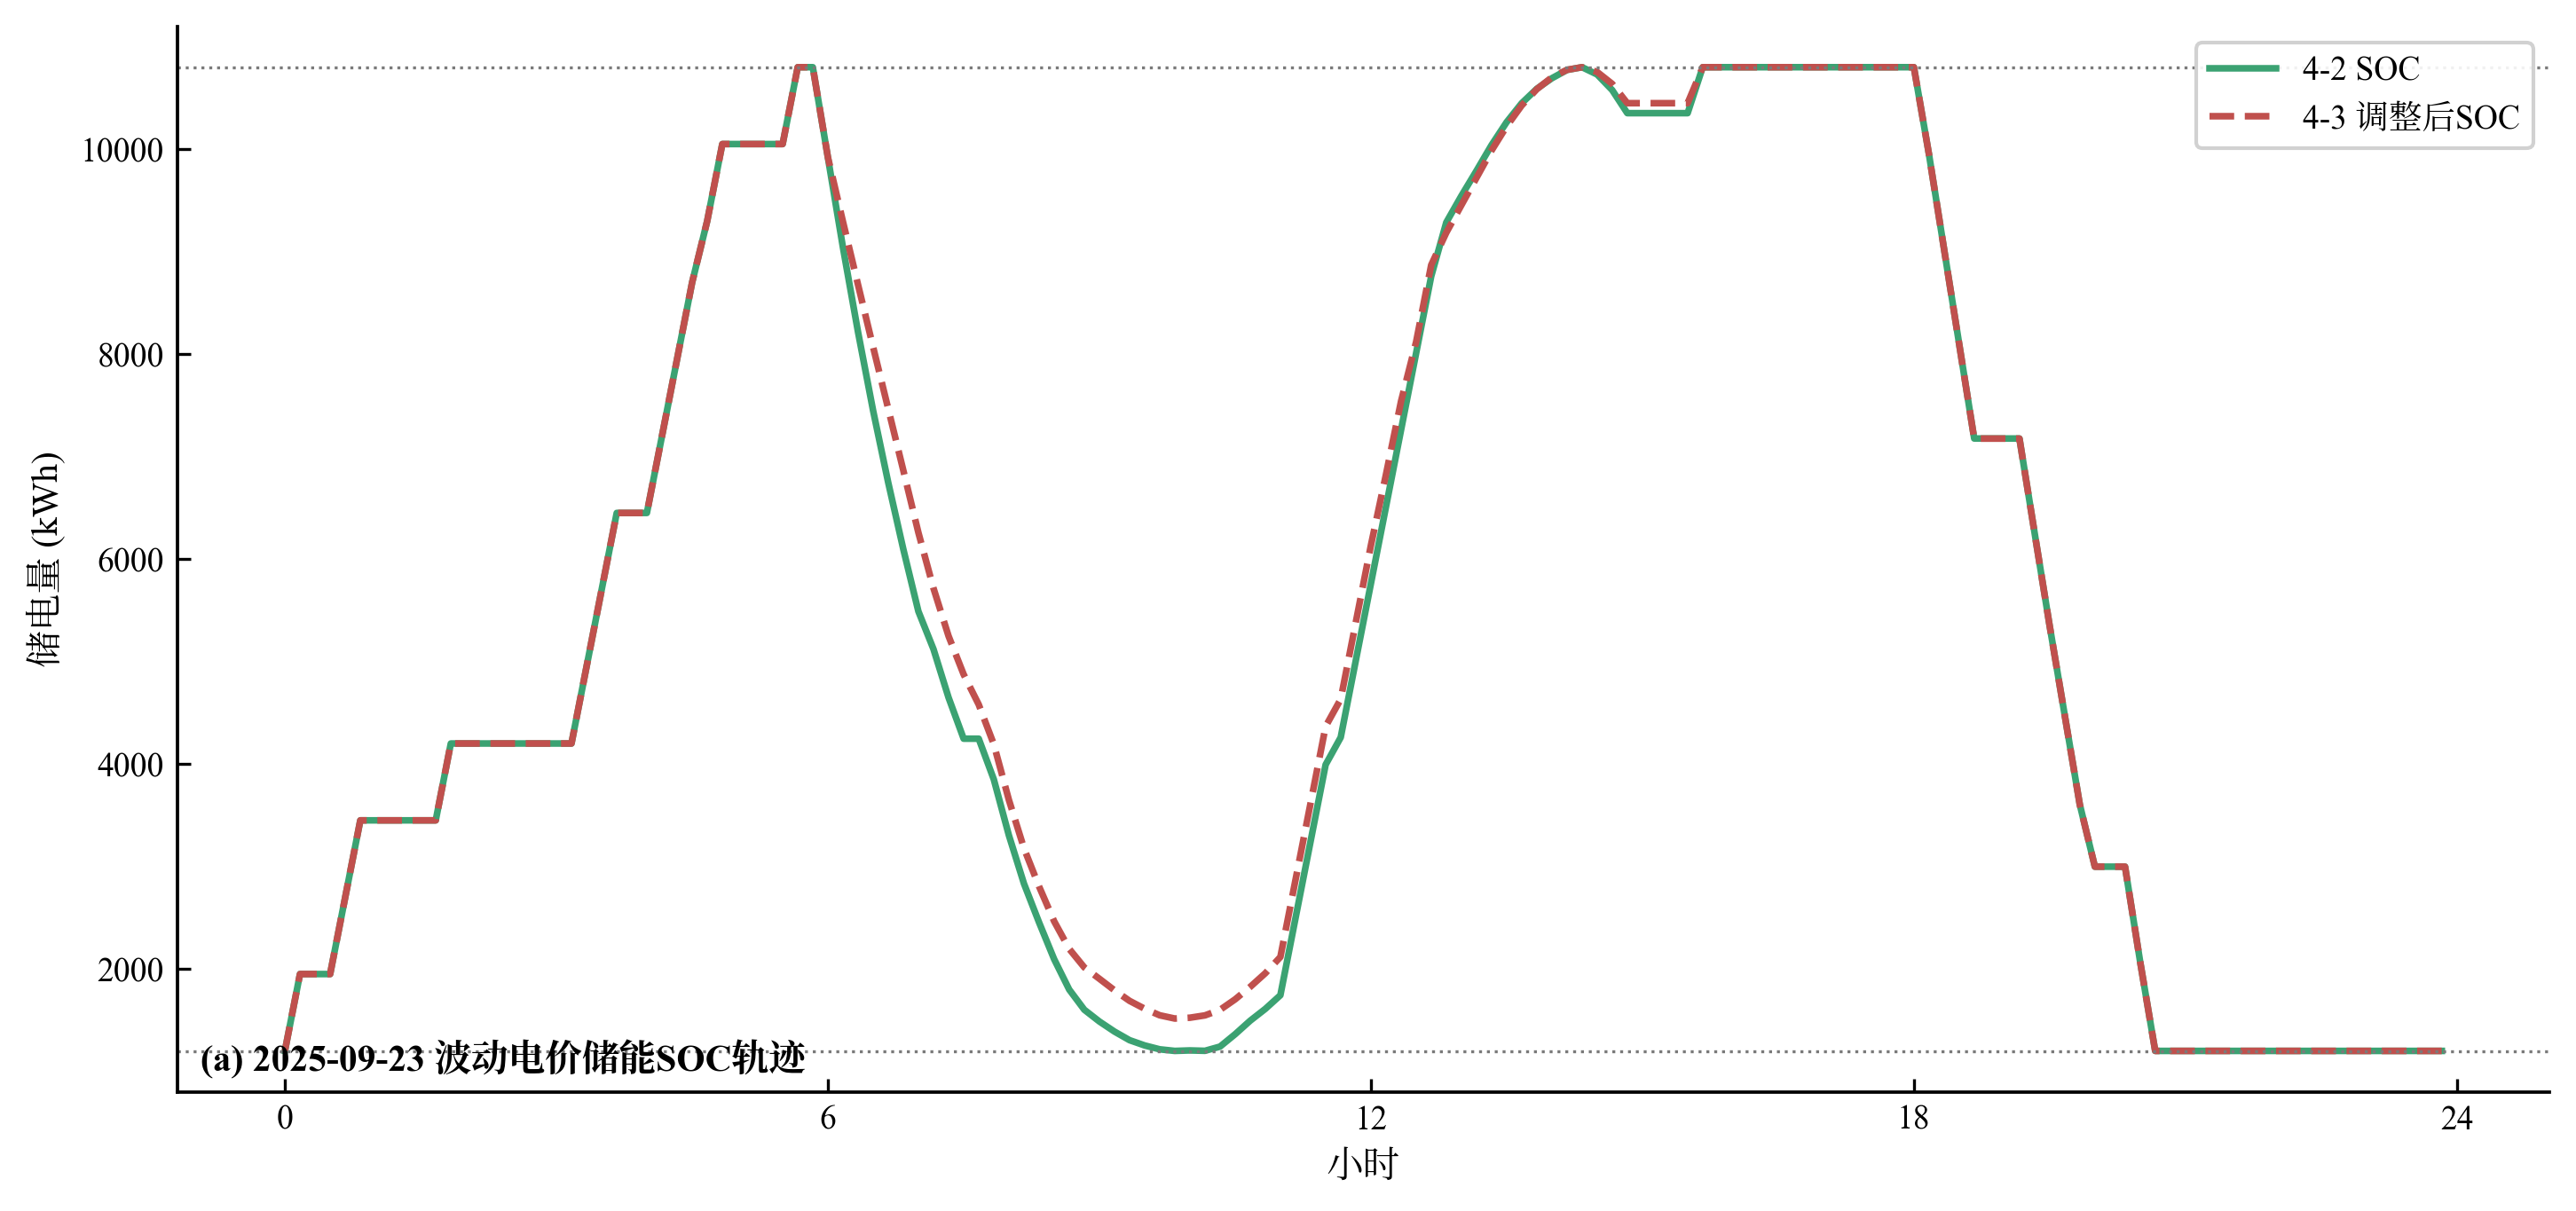
\includegraphics[width=0.70\textwidth]{../求解/问题四/图片/图4-4_波动电价SOC轨迹.png}
    \caption{波动电价下典型日储能荷电状态轨迹}
    \label{fig:结果4-4}
\end{figure}

波动电价下 2.1—12.31 逐日紧急购电量如图\ref{fig:结果4-5}所示。紧急购电量整体保持低位，仅在个别预报偏差较大日期出现尖峰，与固定电价情形的规律一致，说明滚动调整在波动电价下同样有效。

\begin{figure}[H]
    \centering
    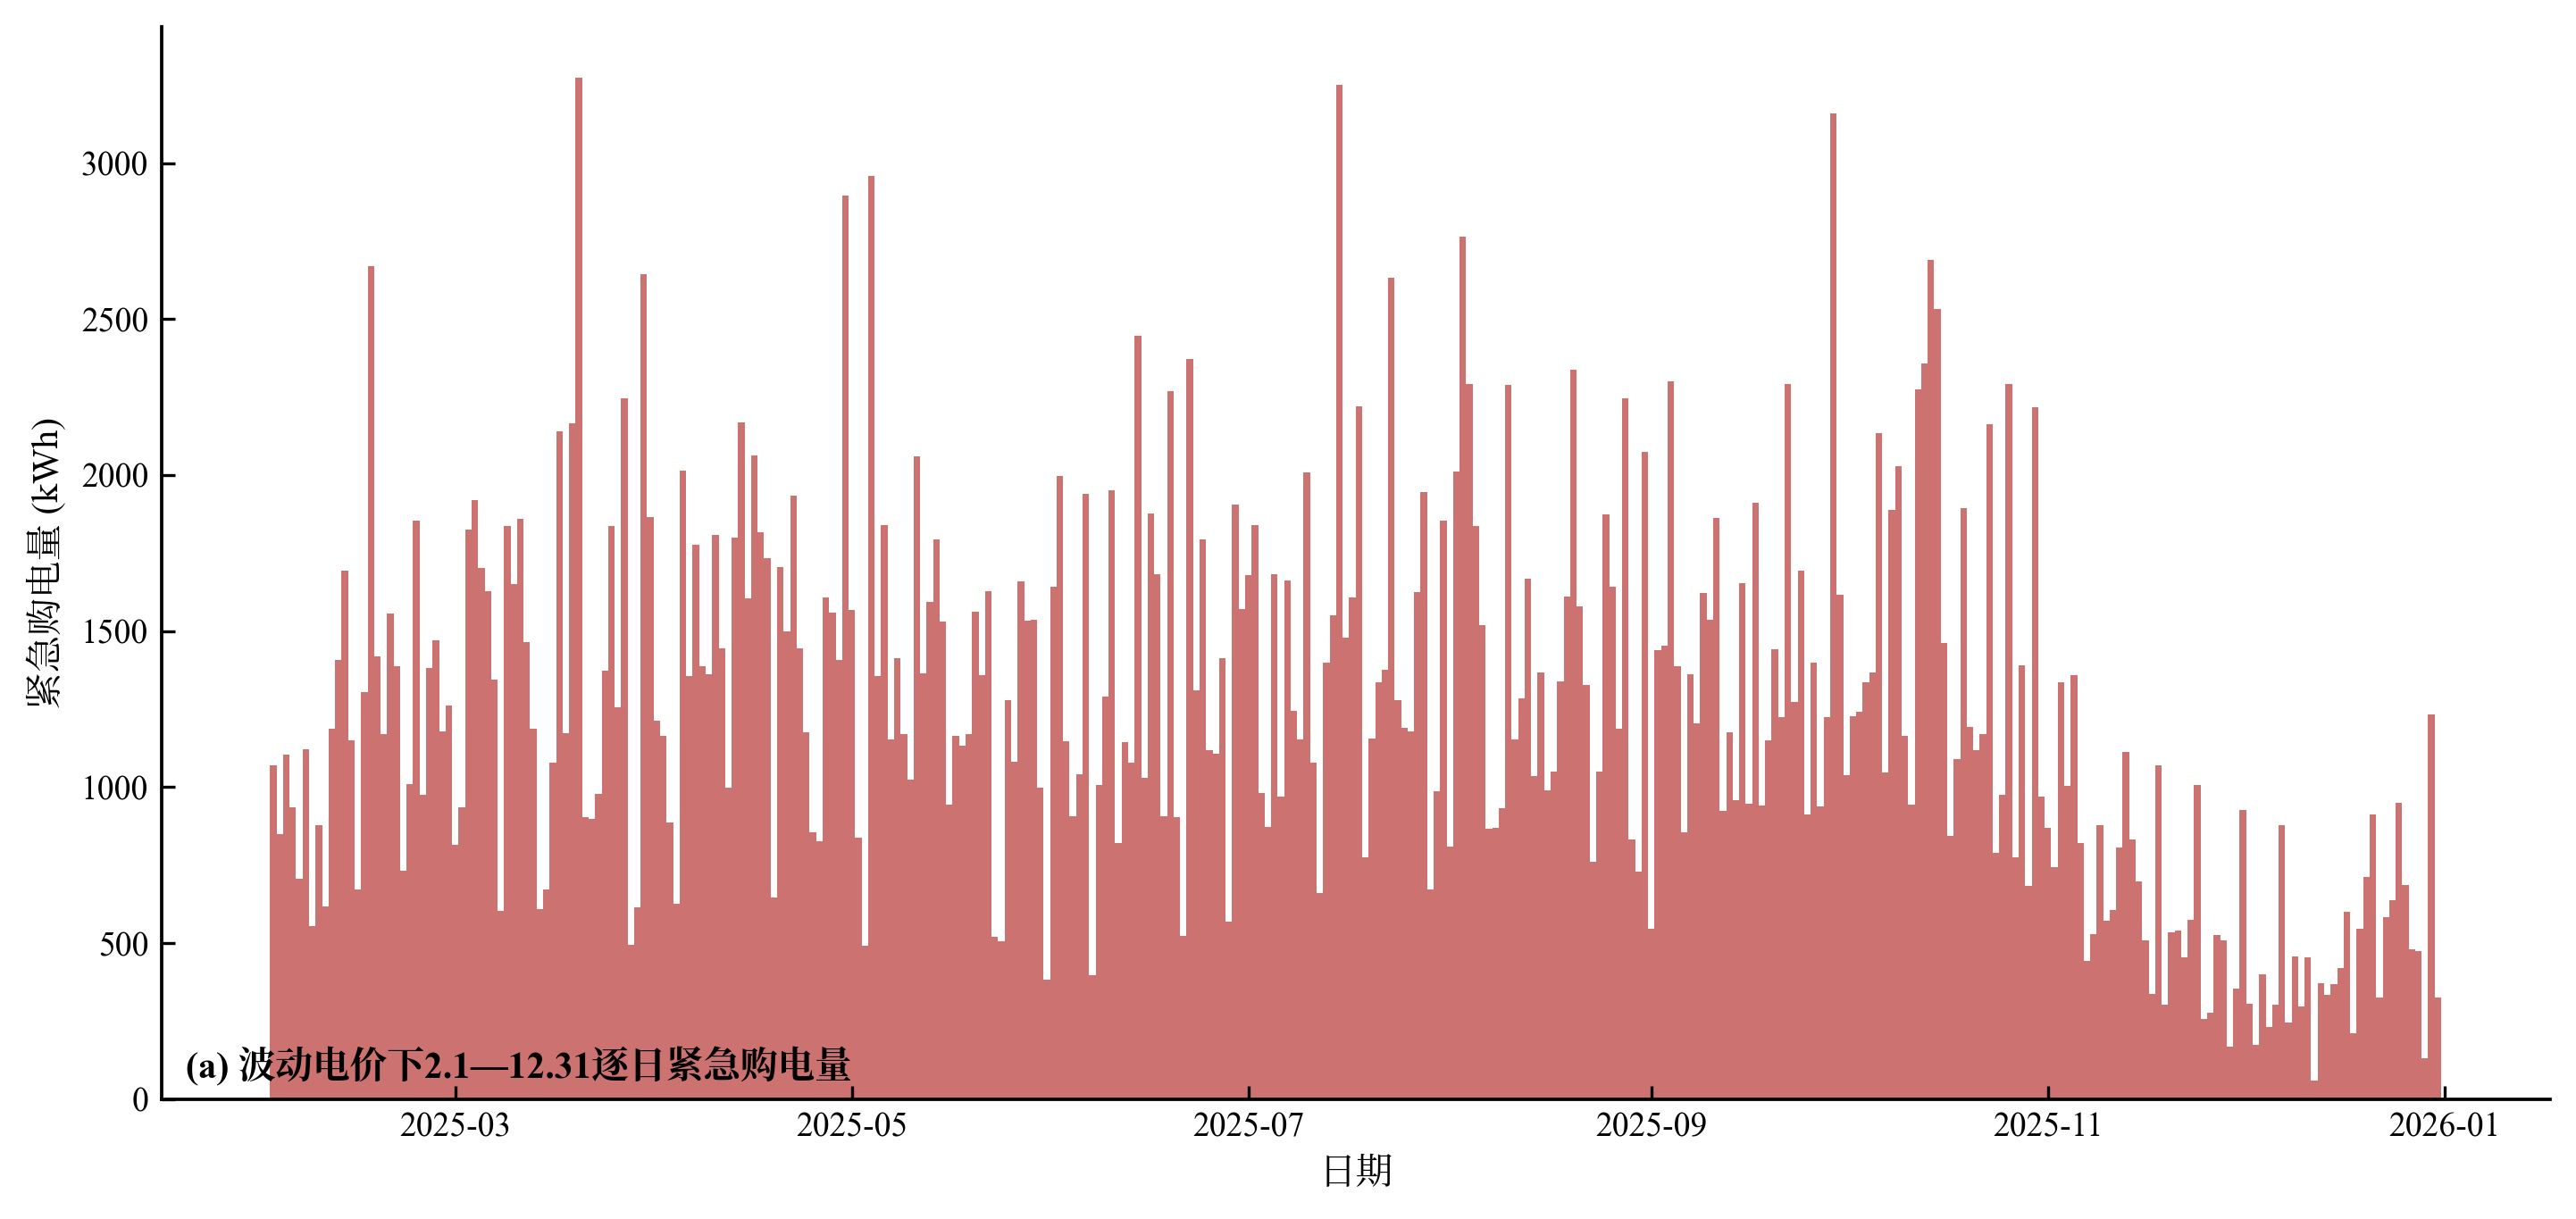
\includegraphics[width=0.70\textwidth]{../求解/问题四/图片/图4-5_波动电价紧急购电量.png}
    \caption{波动电价下2.1—12.31逐日紧急购电量}
    \label{fig:结果4-5}
\end{figure}

固定电价与波动电价下的费用对比如图\ref{fig:结果4-6}所示。波动电价下问题二与问题三的费用均高于固定电价情形，其中问题二由 12254765.72 元升至 12841054.36 元，问题三由 14337999.15 元升至 14956526.18 元，说明实时波动的电价增加了微网购电的不确定性与成本，储能套利只能部分对冲电价波动的影响。

\begin{figure}[H]
    \centering
    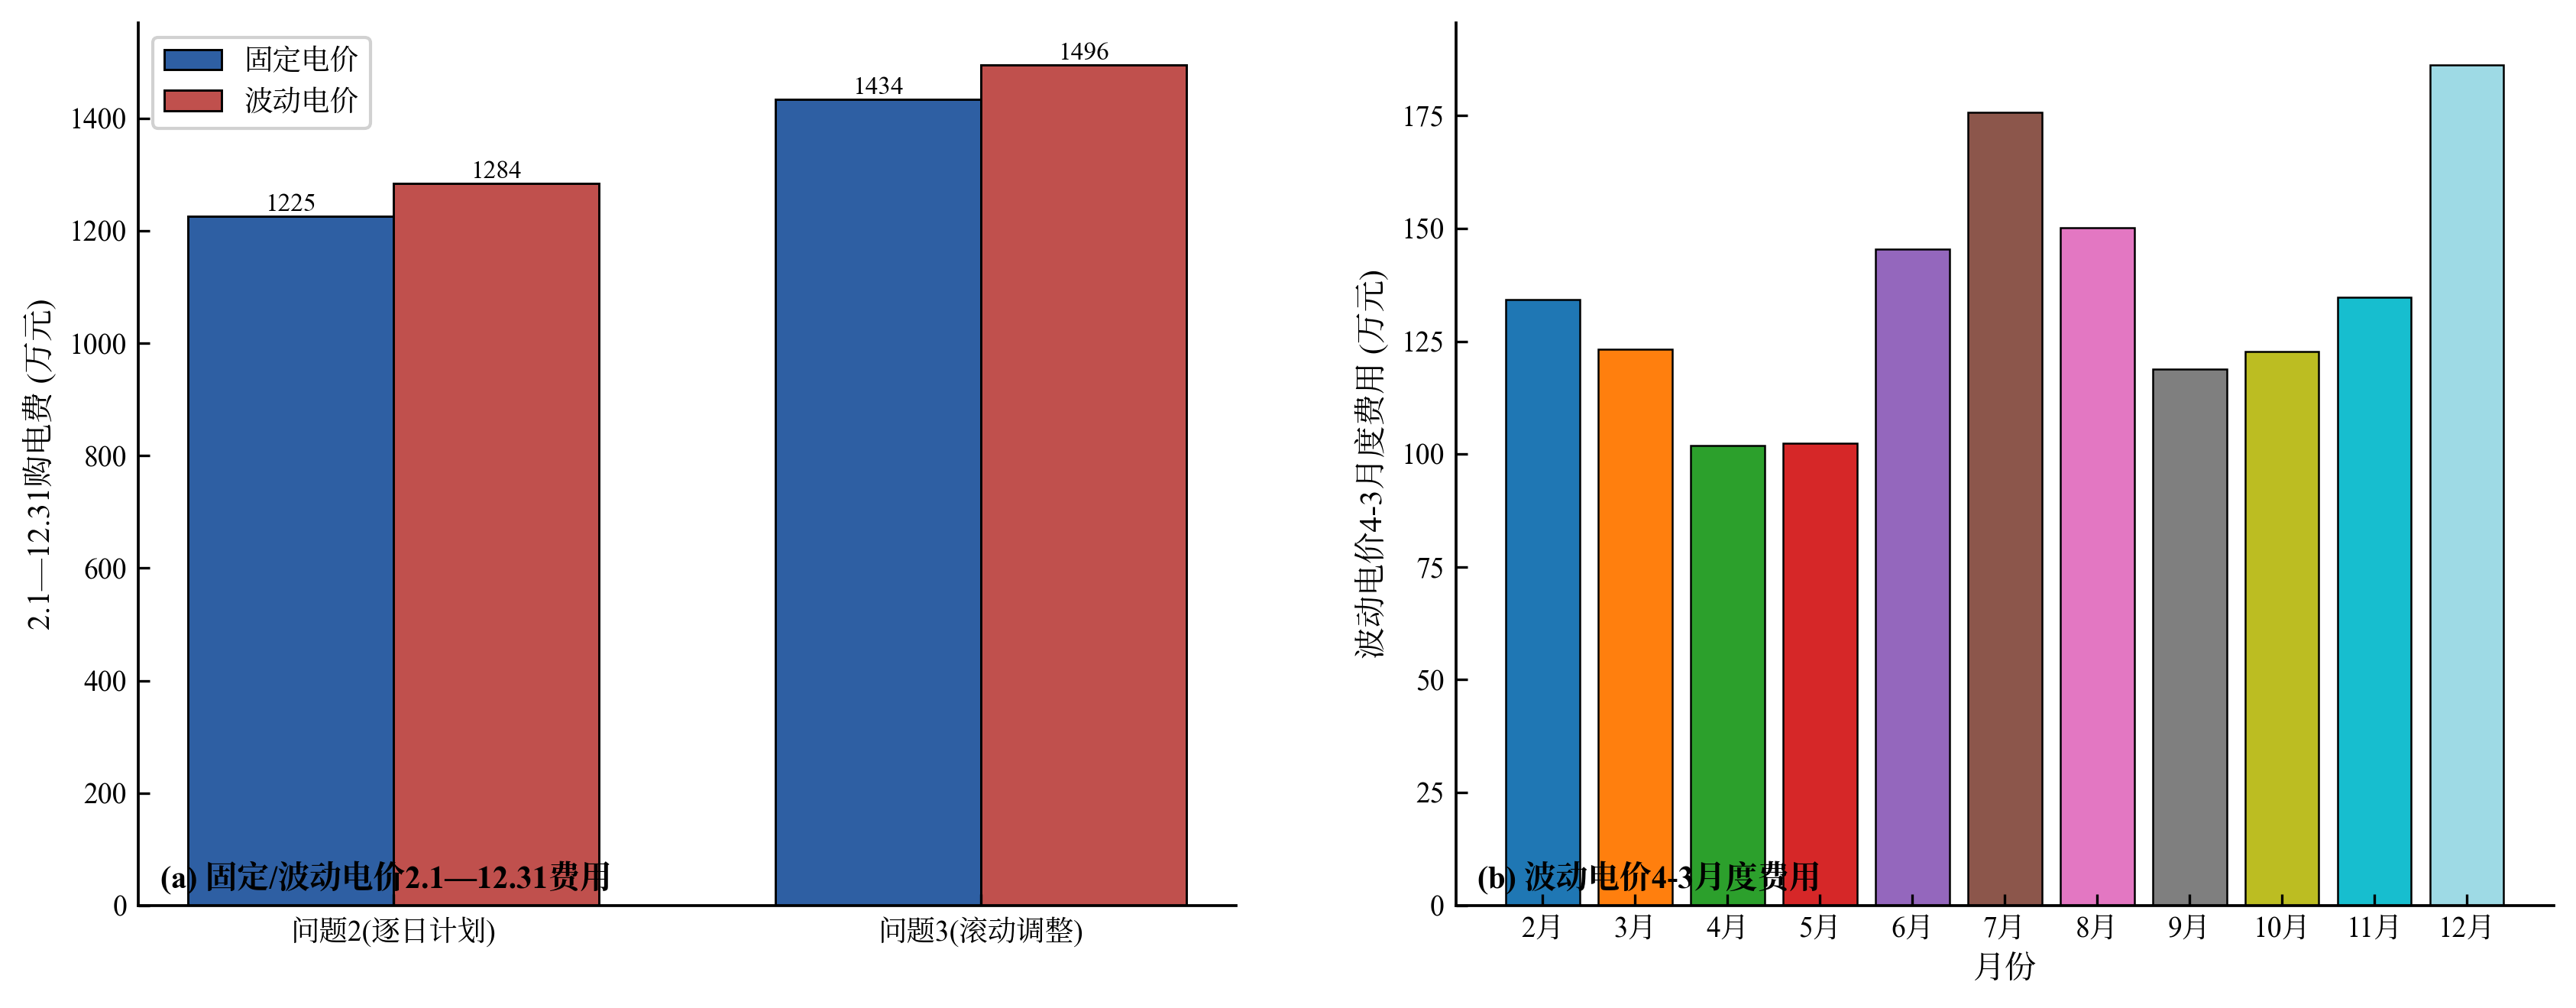
\includegraphics[width=0.72\textwidth]{../求解/问题四/图片/图4-6_固定与波动电价费用对比.png}
    \caption{固定电价与波动电价费用对比（2.1—12.31）}
    \label{fig:结果4-6}
\end{figure}

综合以上结果，问题四在波动电价下重新计算了问题二与问题三的购电策略，两套模型均能稳定运行，储能低充高放的套利行为在波动电价下更为活跃，但购电费用较固定电价情形有所上升，结论合理可靠。
